\section{Additional experiments}
\label{sec:appendix_experiemnt}
This section includes experiments, not in the main paper. 
We first show the comparison of boosting algorithms, 
LPBoost, ERLPBoost, C-ERLPBoost, and our scheme. 
Since C-ERLPBoost is an instance of the short-step FW algorithm, 
we call it FW. 
We call our scheme with secondary algorithm~\ref{alg:lpb_subroutine} 
as MLPBoost. 
Figure~\ref{fig:appendix_margin_objectives} shows the convergence curve. 
MLPB.~(SS) is MLPBoost with FW algorithm~\ref{alg:ss_rule}, 
and MLPB.~(PFW) is MLPBoost 
with Pairwise FW algorithm~\ref{alg:pairwise_rule}. 
As expected, our algorithm converges faster than ERLPBoost 
and is competitive with LPBoost. 
\begin{figure}[p]
    \centering
    \begin{tabular}{ccc}
        \begin{minipage}[t]{0.31\hsize}
            \centering
            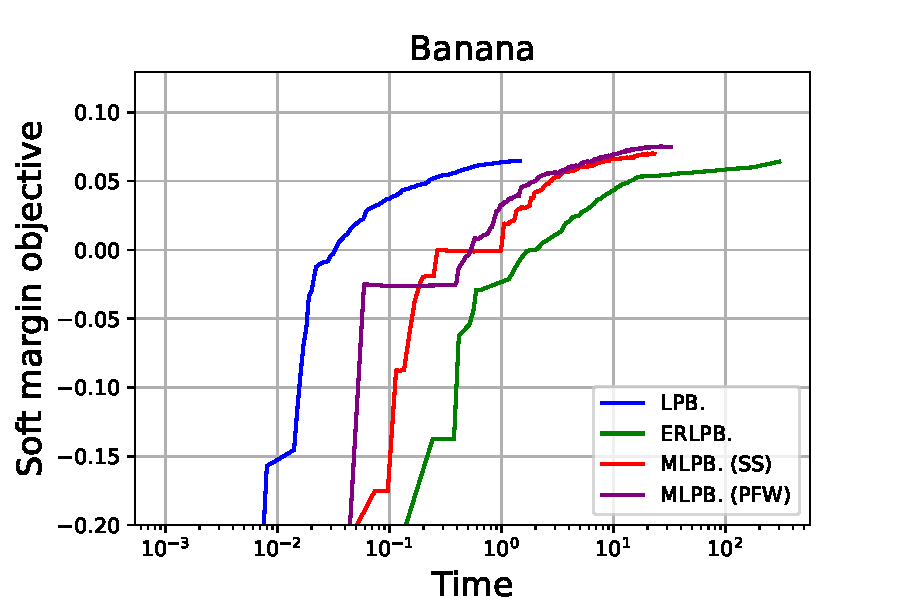
\includegraphics[keepaspectratio, scale=0.30]
            {figure/curve_logtime_banana.pdf}
        \end{minipage}
        &
        \begin{minipage}[t]{0.31\hsize}
            \centering
            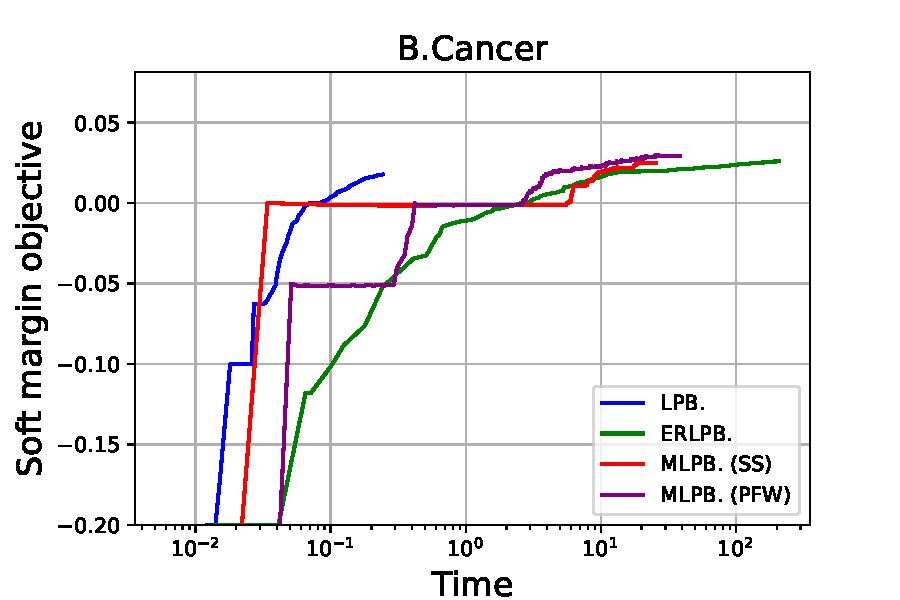
\includegraphics[keepaspectratio, scale=0.30]
            {figure/curve_logtime_breast_cancer.pdf}
        \end{minipage}
        &
        \begin{minipage}[t]{0.31\hsize}
            \centering
            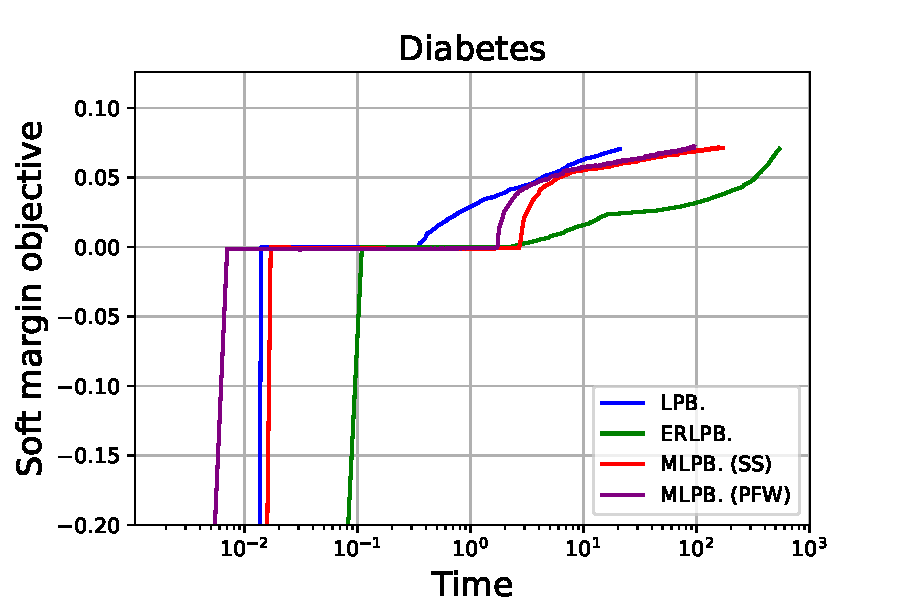
\includegraphics[keepaspectratio, scale=0.30]
            {figure/curve_logtime_diabetis.pdf}
        \end{minipage}
        \\
        \begin{minipage}[t]{0.31\hsize}
            \centering
            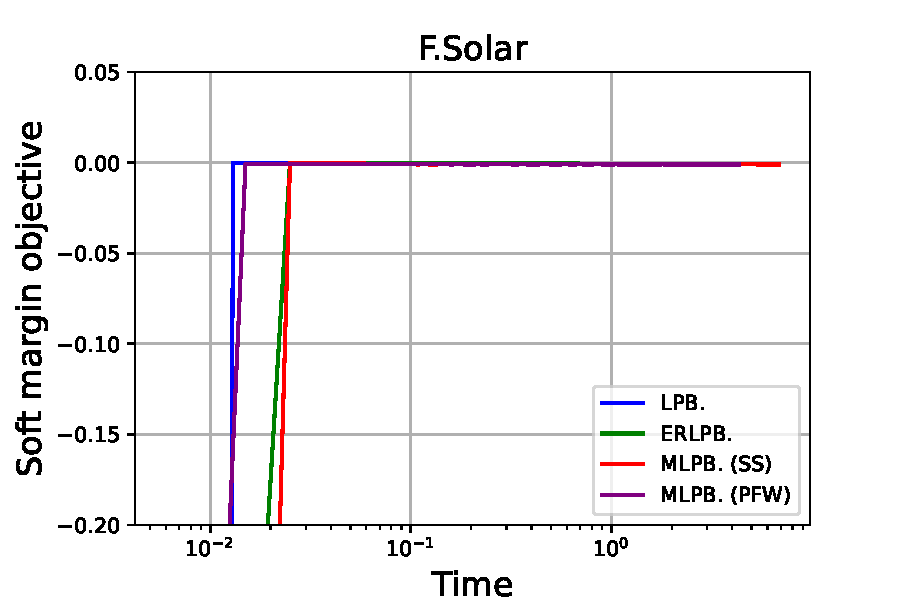
\includegraphics[keepaspectratio, scale=0.30]
            {figure/curve_logtime_flare_solar.pdf}
        \end{minipage}
        &
        \begin{minipage}[t]{0.31\hsize}
            \centering
            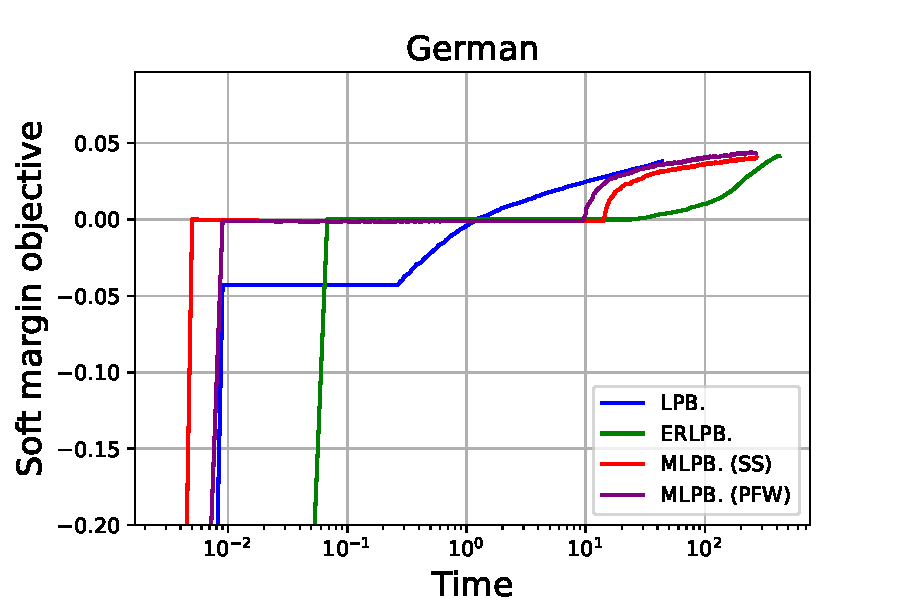
\includegraphics[keepaspectratio, scale=0.30]
            {figure/curve_logtime_german.pdf}
        \end{minipage}
        &
        \begin{minipage}[t]{0.31\hsize}
            \centering
            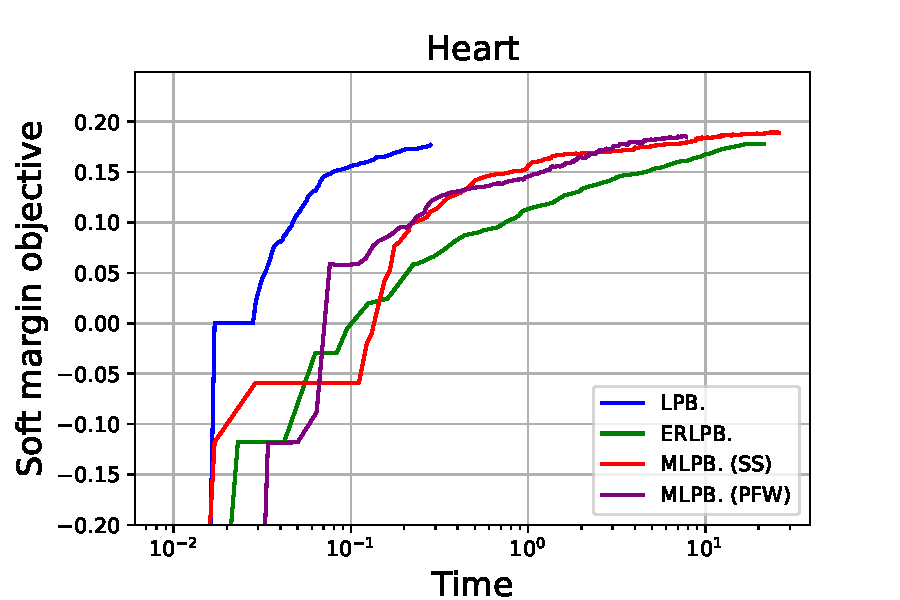
\includegraphics[keepaspectratio, scale=0.30]
            {figure/curve_logtime_heart.pdf}
        \end{minipage}
        \\
        \begin{minipage}[t]{0.31\hsize}
            \centering
            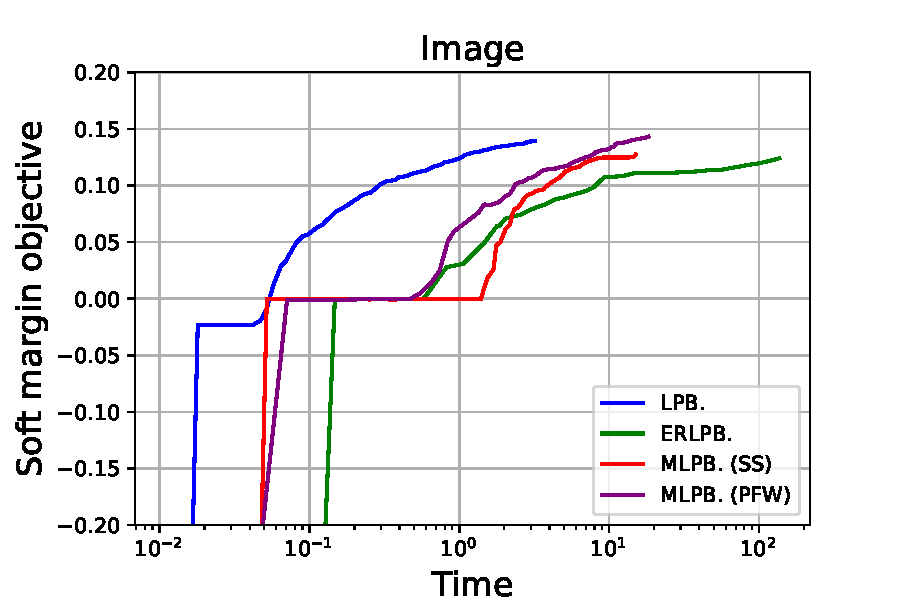
\includegraphics[keepaspectratio, scale=0.30]
            {figure/curve_logtime_image.pdf}
        \end{minipage}
        &
        \begin{minipage}[t]{0.31\hsize}
            \centering
            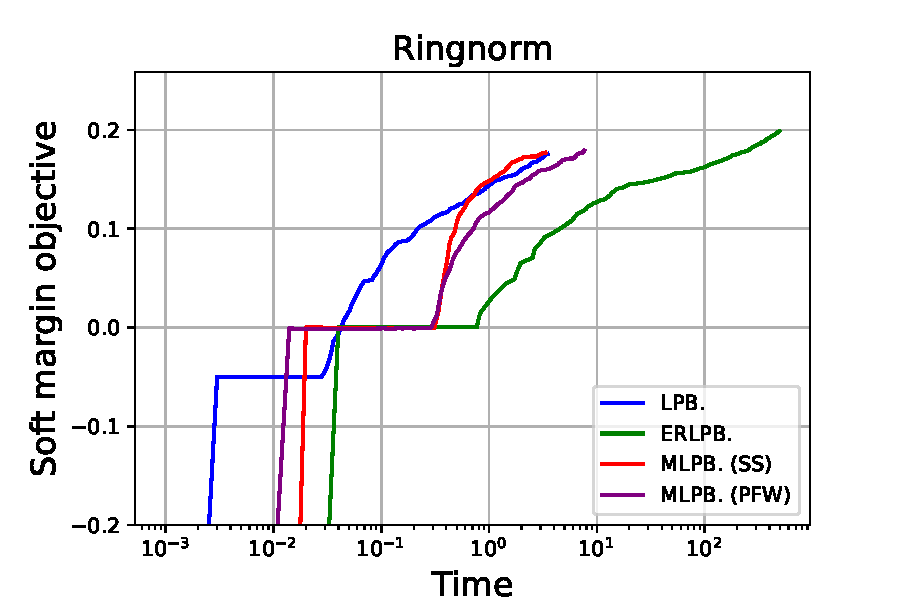
\includegraphics[keepaspectratio, scale=0.30]
            {figure/curve_logtime_ringnorm.pdf}
        \end{minipage}
        &
        \begin{minipage}[t]{0.31\hsize}
            \centering
            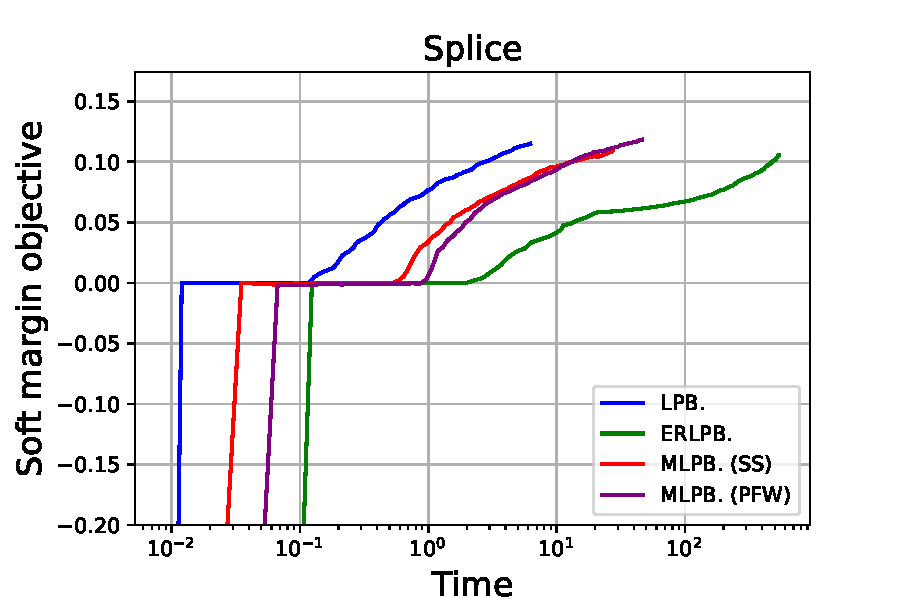
\includegraphics[keepaspectratio, scale=0.30]
            {figure/curve_logtime_splice.pdf}
        \end{minipage}
        \\
        \begin{minipage}[t]{0.31\hsize}
            \centering
            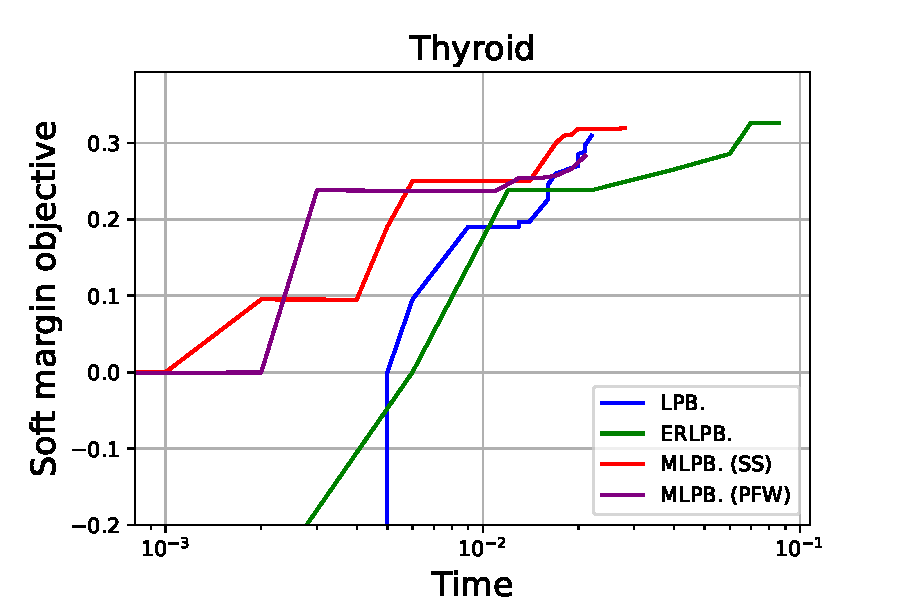
\includegraphics[keepaspectratio, scale=0.30]
            {figure/curve_logtime_thyroid.pdf}
        \end{minipage}
        &
        \begin{minipage}[t]{0.31\hsize}
            \centering
            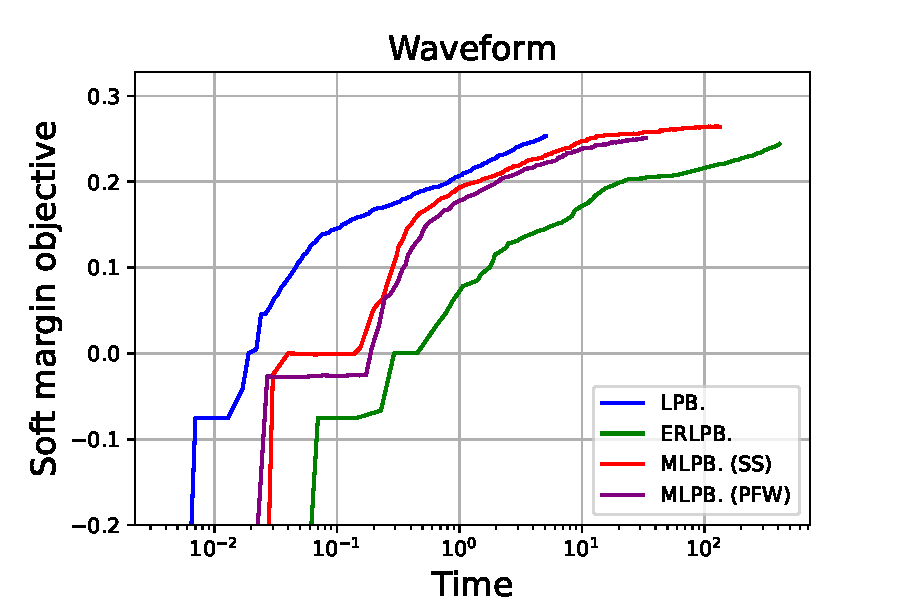
\includegraphics[keepaspectratio, scale=0.30]
            {figure/curve_logtime_waveform.pdf}
        \end{minipage}
        &
        \begin{minipage}[t]{0.31\hsize}
            \centering
            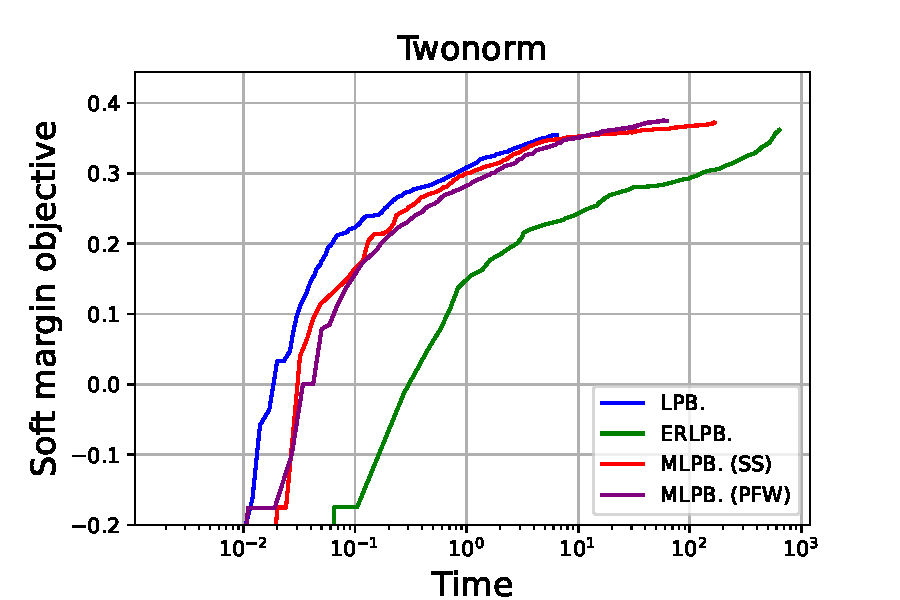
\includegraphics[keepaspectratio, scale=0.30]
            {figure/curve_logtime_twonorm.pdf}
        \end{minipage}
    \end{tabular}
    \caption{%
        Time vs. soft margin objective %
        with parameters $\nu = 0.1m$ and $\epsilon = 0.01$. %
        Note that the time axis is log-scale. %
        For many datasets, MLPBoosts tend to achieve %
        a large margin rapidly. %
    }
    \label{fig:appendix_margin_objectives}
\end{figure}

Further, we compare the test error decrease. 
Figure~\ref{fig:appendix_test_errors} shows the test error curves. 
MLPB.~(SS) achieves low test errors in most datasets. 
\begin{figure}[p]
    \centering
    \begin{tabular}{ccc}
        \begin{minipage}[t]{0.31\hsize}
            \centering
            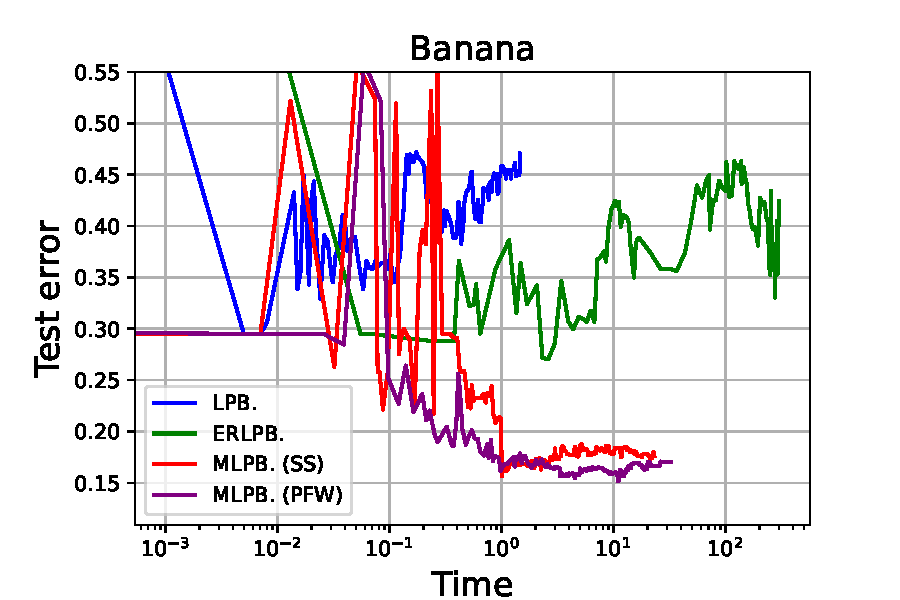
\includegraphics[keepaspectratio, scale=0.30]
            {figure/test_logtime_banana.pdf}
        \end{minipage}
        &
        \begin{minipage}[t]{0.31\hsize}
            \centering
            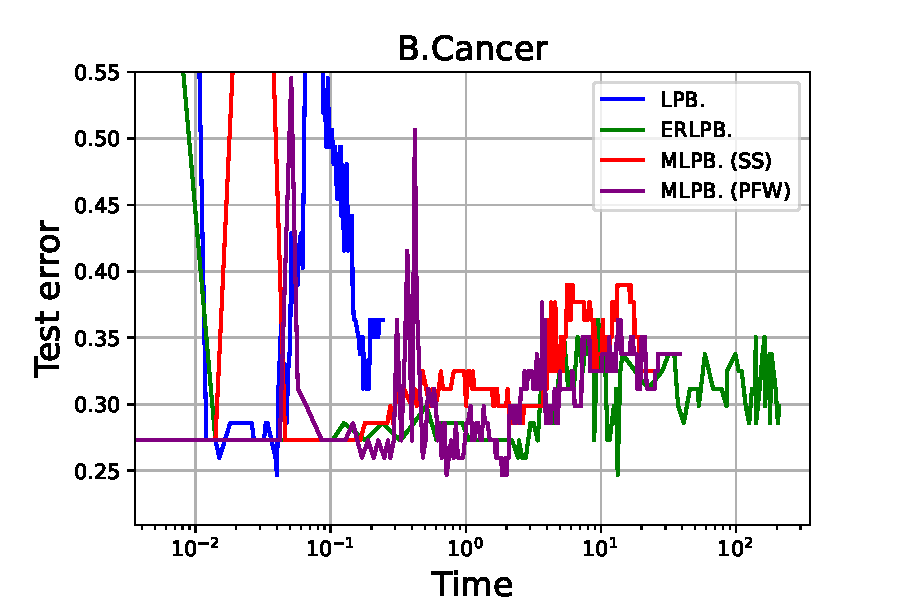
\includegraphics[keepaspectratio, scale=0.30]
            {figure/test_logtime_breast_cancer.pdf}
        \end{minipage}
        &
        \begin{minipage}[t]{0.31\hsize}
            \centering
            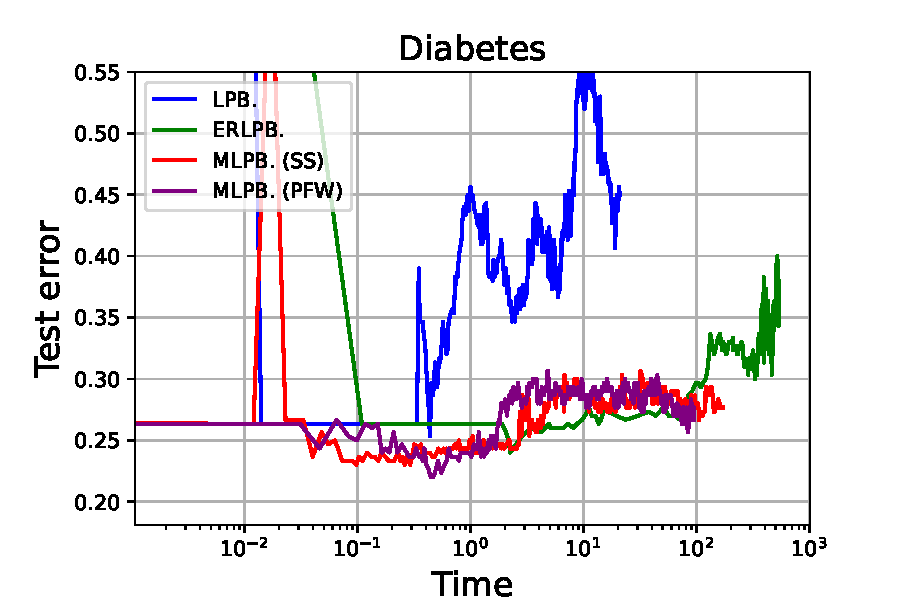
\includegraphics[keepaspectratio, scale=0.30]
            {figure/test_logtime_diabetis.pdf}
        \end{minipage}
        \\
        \begin{minipage}[t]{0.31\hsize}
            \centering
            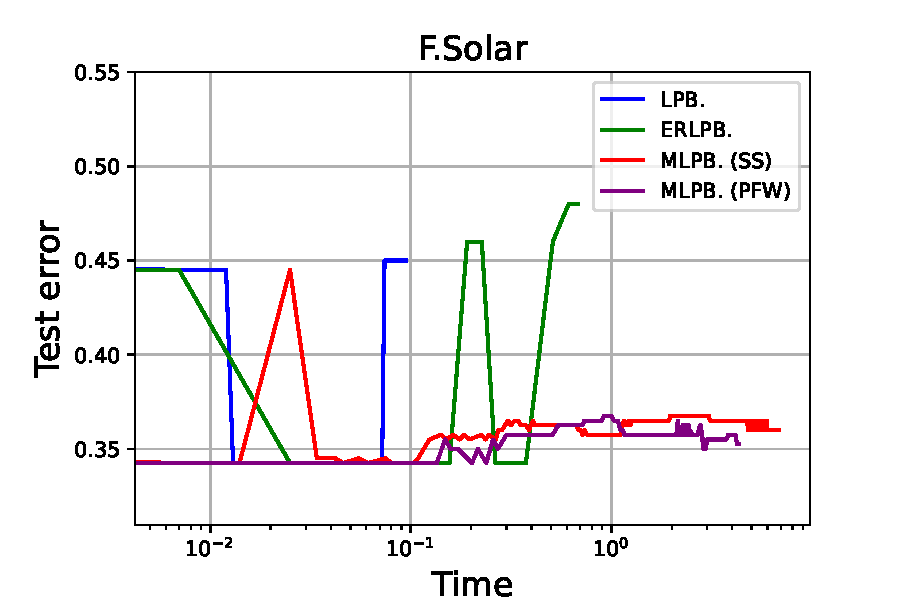
\includegraphics[keepaspectratio, scale=0.30]
            {figure/test_logtime_flare_solar.pdf}
        \end{minipage}
        &
        \begin{minipage}[t]{0.31\hsize}
            \centering
            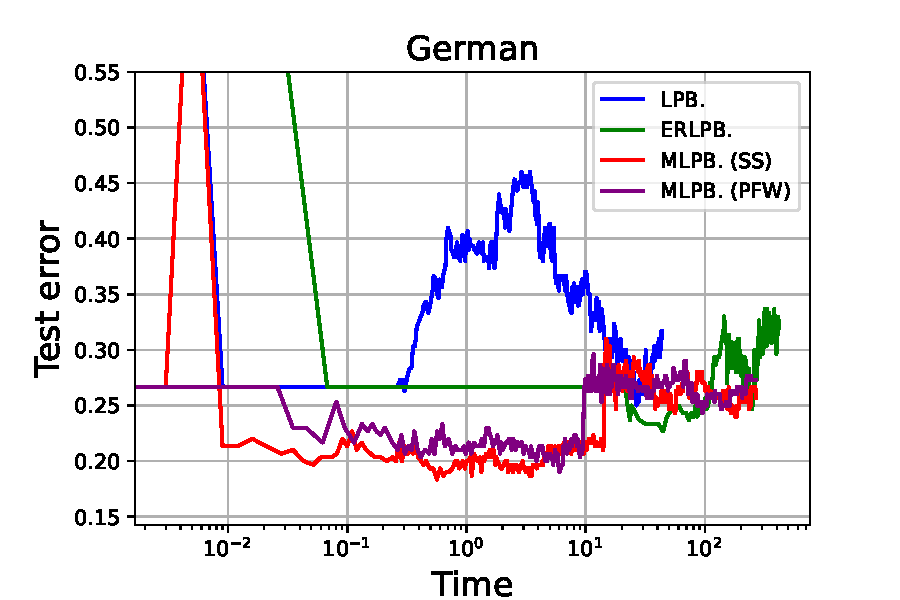
\includegraphics[keepaspectratio, scale=0.30]
            {figure/test_logtime_german.pdf}
        \end{minipage}
        &
        \begin{minipage}[t]{0.31\hsize}
            \centering
            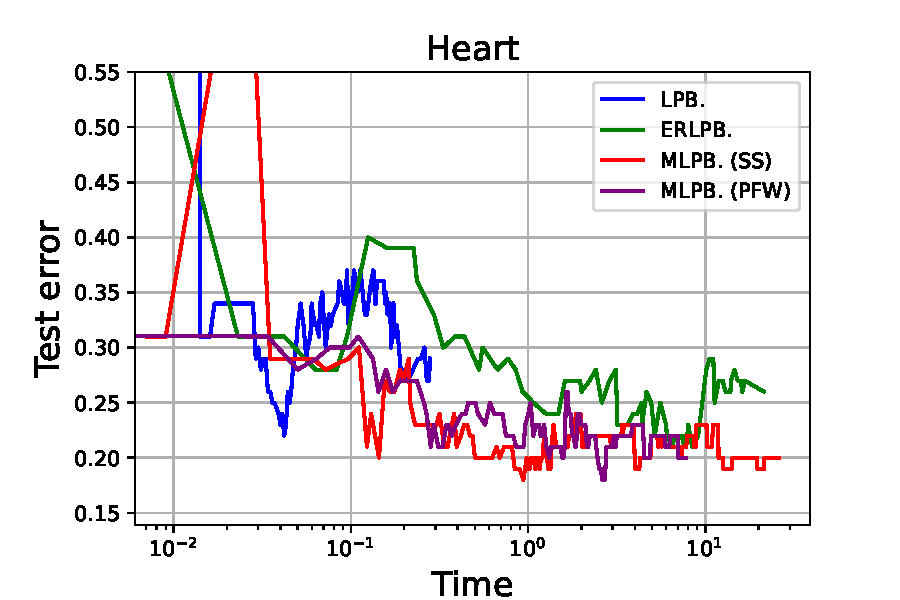
\includegraphics[keepaspectratio, scale=0.30]
            {figure/test_logtime_heart.pdf}
        \end{minipage}
        \\
        \begin{minipage}[t]{0.31\hsize}
            \centering
            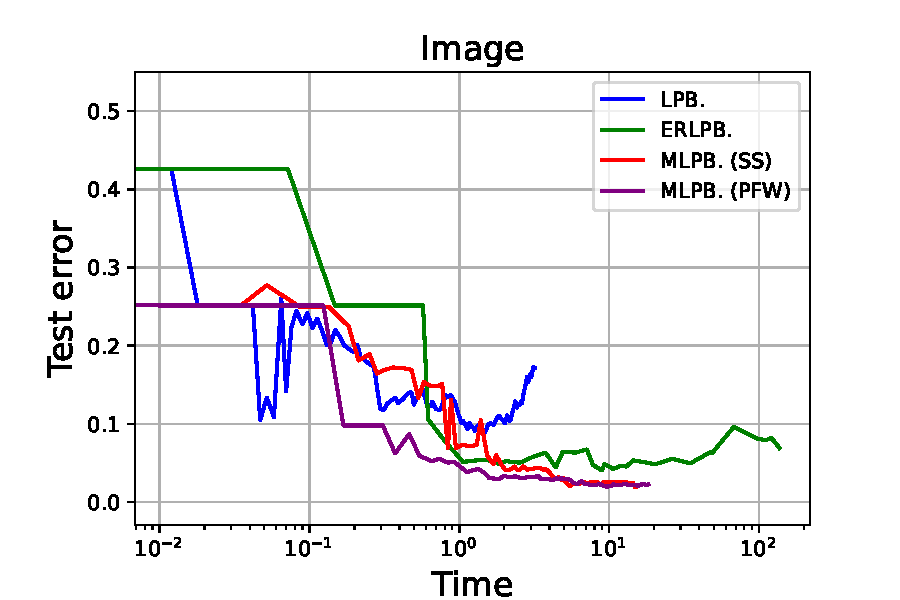
\includegraphics[keepaspectratio, scale=0.30]
            {figure/test_logtime_image.pdf}
        \end{minipage}
        &
        \begin{minipage}[t]{0.31\hsize}
            \centering
            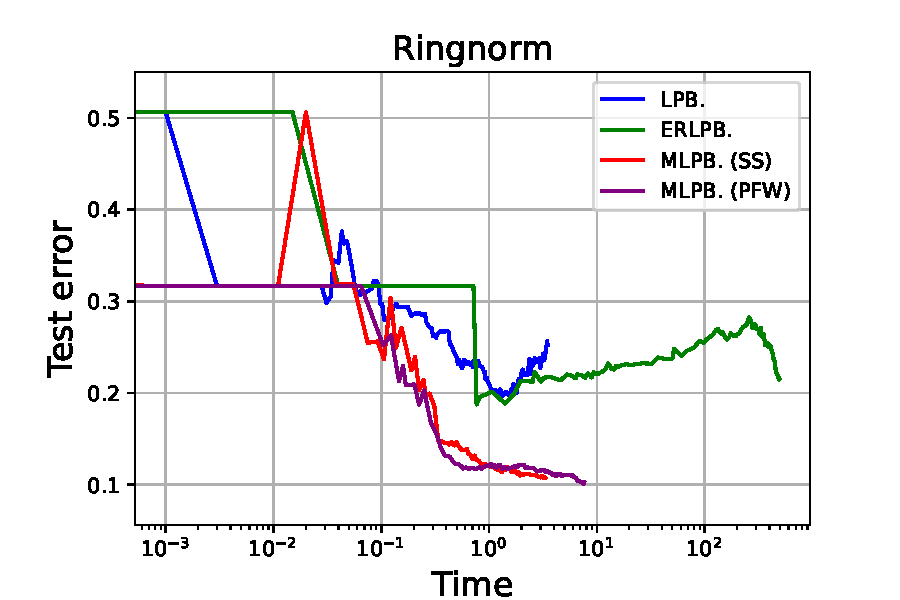
\includegraphics[keepaspectratio, scale=0.30]
            {figure/test_logtime_ringnorm.pdf}
        \end{minipage}
        &
        \begin{minipage}[t]{0.31\hsize}
            \centering
            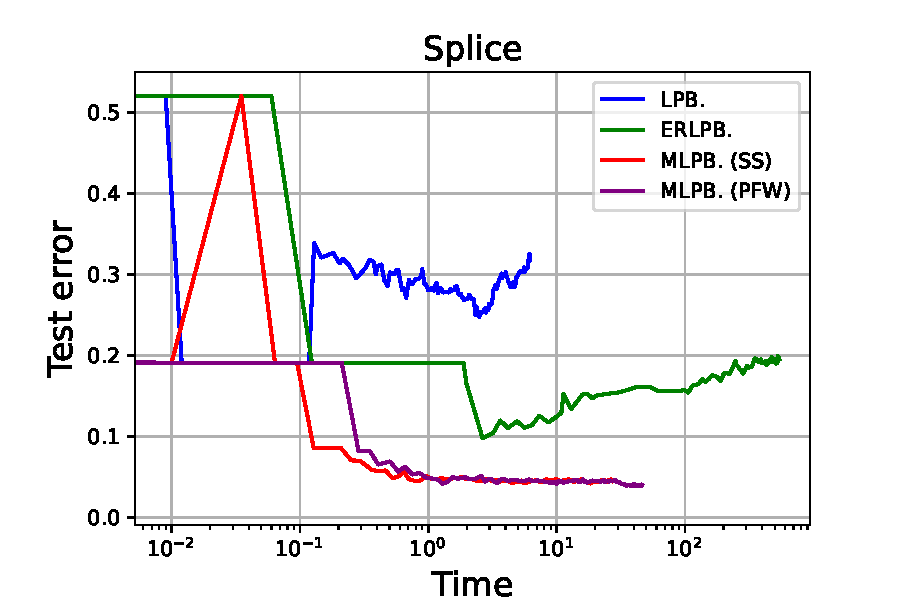
\includegraphics[keepaspectratio, scale=0.30]
            {figure/test_logtime_splice.pdf}
        \end{minipage}
        \\
        \begin{minipage}[t]{0.31\hsize}
            \centering
            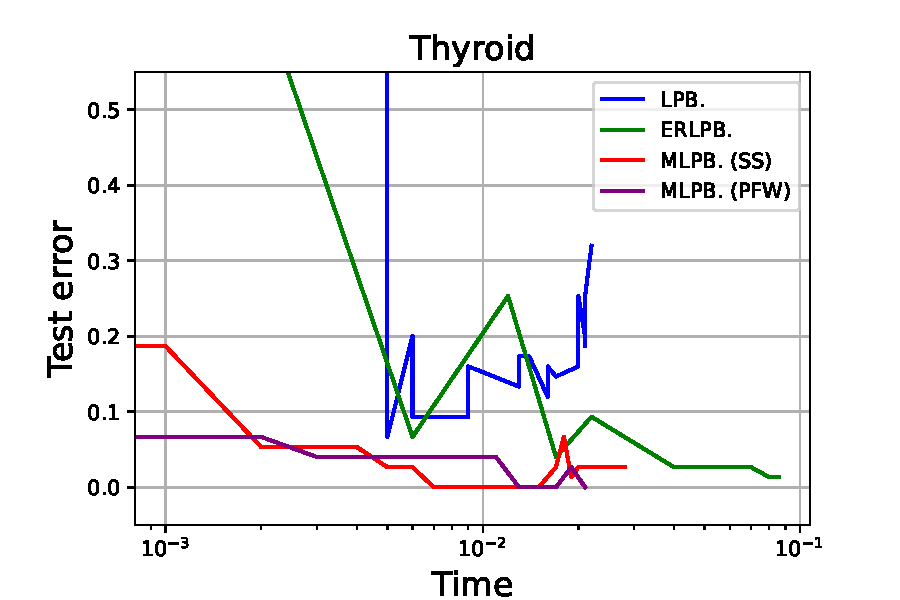
\includegraphics[keepaspectratio, scale=0.30]
            {figure/test_logtime_thyroid.pdf}
        \end{minipage}
        &
        \begin{minipage}[t]{0.31\hsize}
            \centering
            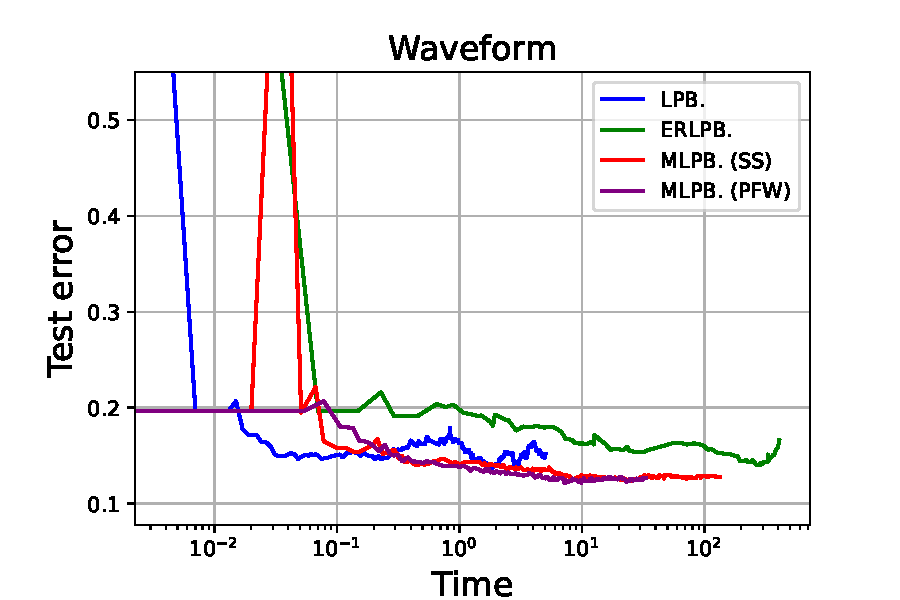
\includegraphics[keepaspectratio, scale=0.30]
            {figure/test_logtime_waveform.pdf}
        \end{minipage}
        &
        \begin{minipage}[t]{0.31\hsize}
            \centering
            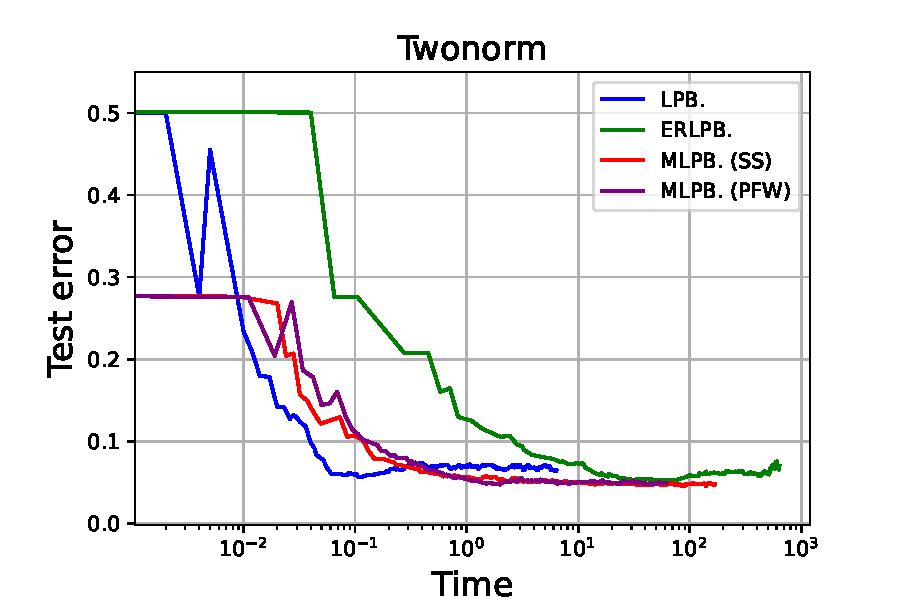
\includegraphics[keepaspectratio, scale=0.30]
            {figure/test_logtime_twonorm.pdf}
        \end{minipage}
    \end{tabular}
    \caption{%
        Time vs. test errors for the 0th fold of each dataset %
        with parameters $\nu = 0.1m$ and $\epsilon = 0.01$. %
        Note that the time axis is log-scale. %
        For many datasets, MLPBoost tends to decrease %
        the test error. %
    }
    \label{fig:appendix_test_errors}
\end{figure}

Now, we compare MLPBoosts to the Frank-Wolfe algorithms, FW and PFW. 
Figure~\ref{fig:appendix_lpbcall} shows 
the number of $\secalg$ updates. 
This figure shows that 
the secondary update $\secalg$ yields better progress 
in early iterations. In the latter half, 
$\fwalg$ yields better progress. 
\begin{figure}[p]
    \centering
    \begin{tabular}{ccc}
        \begin{minipage}[t]{0.31\hsize}
            \centering
            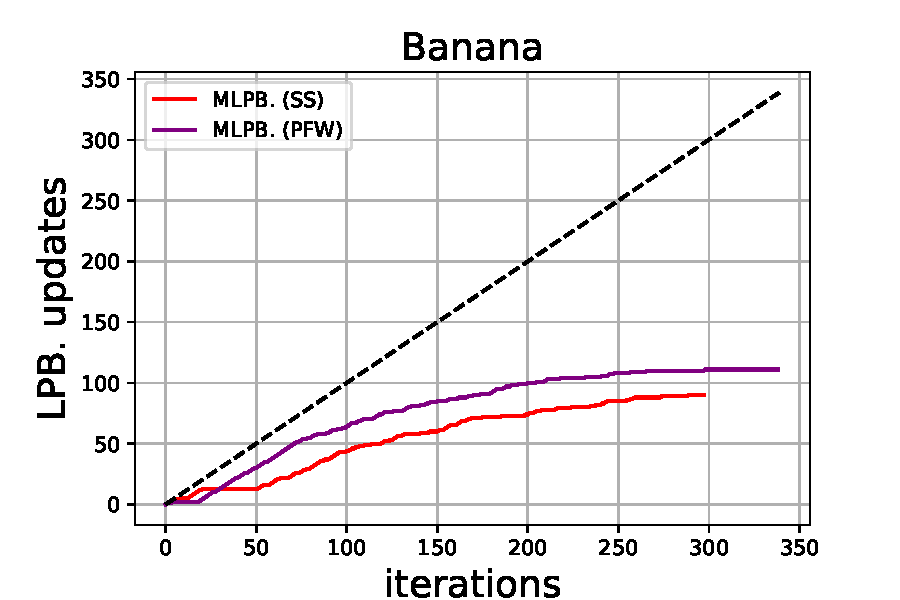
\includegraphics[keepaspectratio, scale=0.30]
            {figure/mlpb_lpb_update_banana.pdf}
        \end{minipage}
        &
        \begin{minipage}[t]{0.31\hsize}
            \centering
            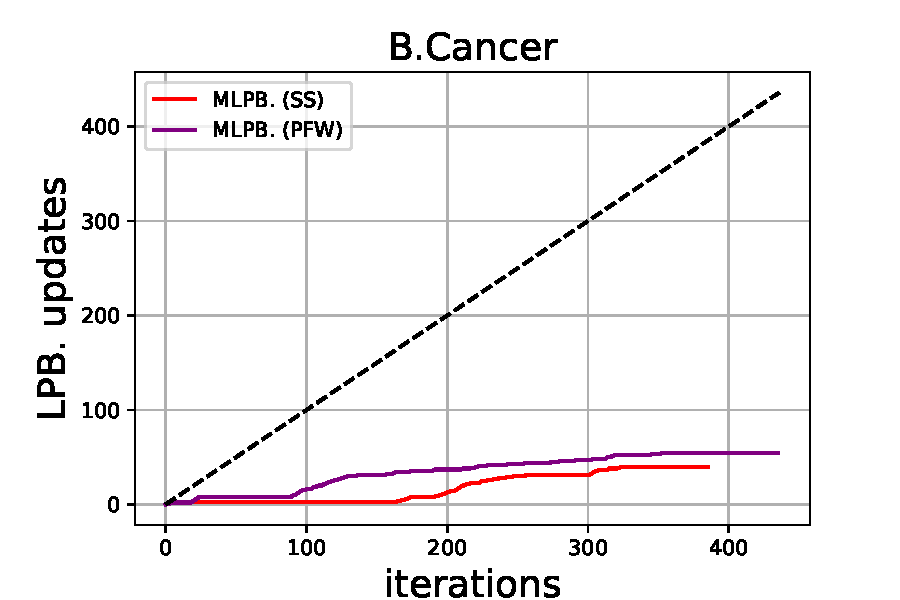
\includegraphics[keepaspectratio, scale=0.30]
            {figure/mlpb_lpb_update_breast_cancer.pdf}
        \end{minipage}
        &
        \begin{minipage}[t]{0.31\hsize}
            \centering
            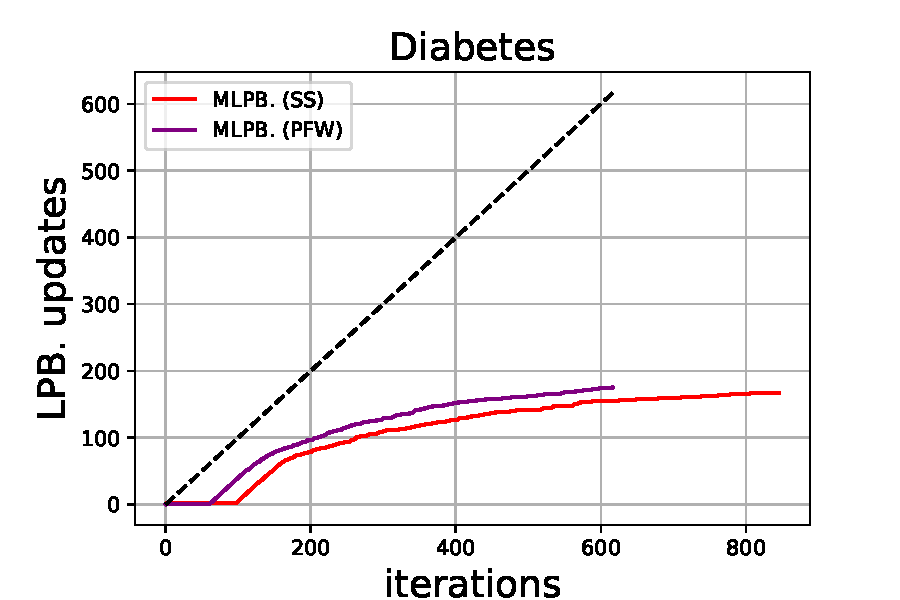
\includegraphics[keepaspectratio, scale=0.30]
            {figure/mlpb_lpb_update_diabetis.pdf}
        \end{minipage}
        \\
        \begin{minipage}[t]{0.31\hsize}
            \centering
            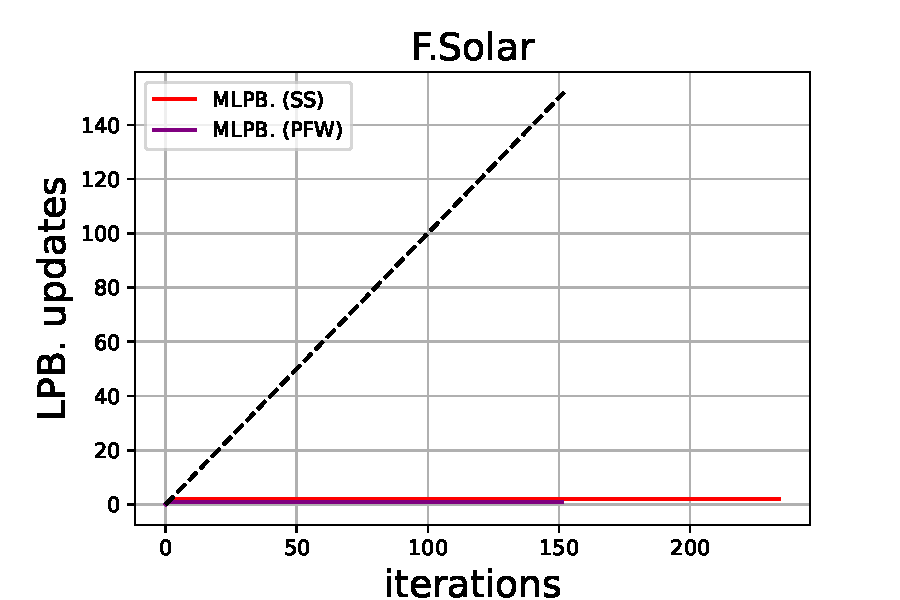
\includegraphics[keepaspectratio, scale=0.30]
            {figure/mlpb_lpb_update_flare_solar.pdf}
        \end{minipage}
        &
        \begin{minipage}[t]{0.31\hsize}
            \centering
            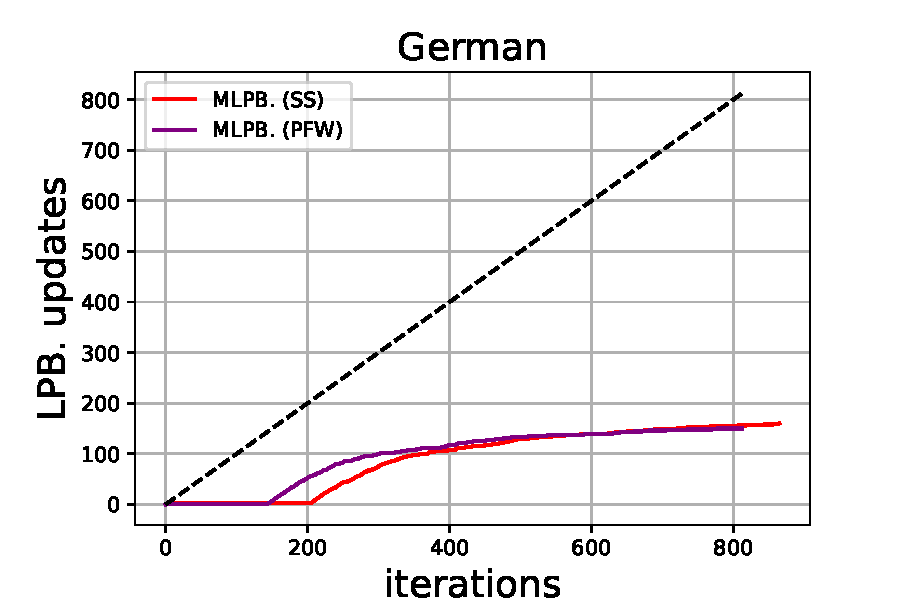
\includegraphics[keepaspectratio, scale=0.30]
            {figure/mlpb_lpb_update_german.pdf}
        \end{minipage}
        &
        \begin{minipage}[t]{0.31\hsize}
            \centering
            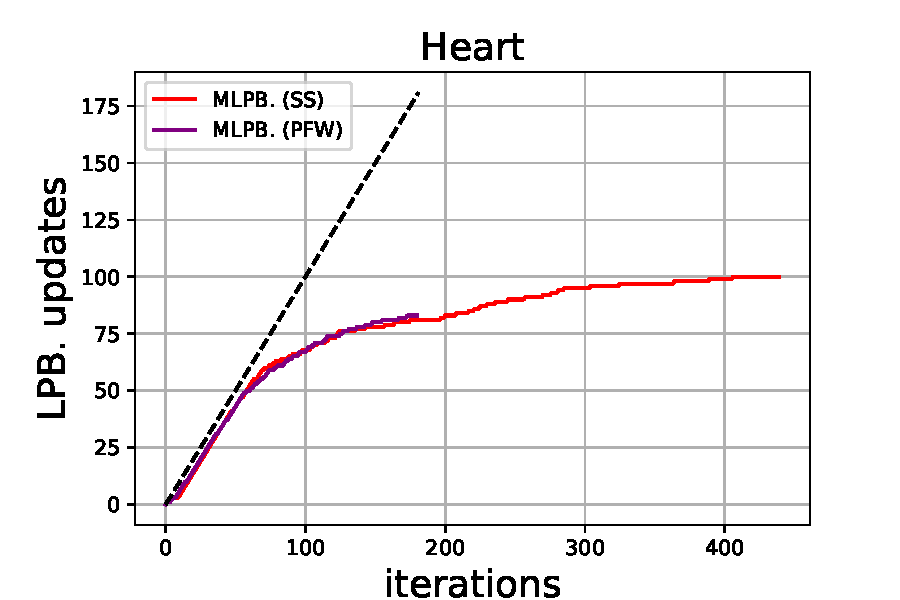
\includegraphics[keepaspectratio, scale=0.30]
            {figure/mlpb_lpb_update_heart.pdf}
        \end{minipage}
        \\
        \begin{minipage}[t]{0.31\hsize}
            \centering
            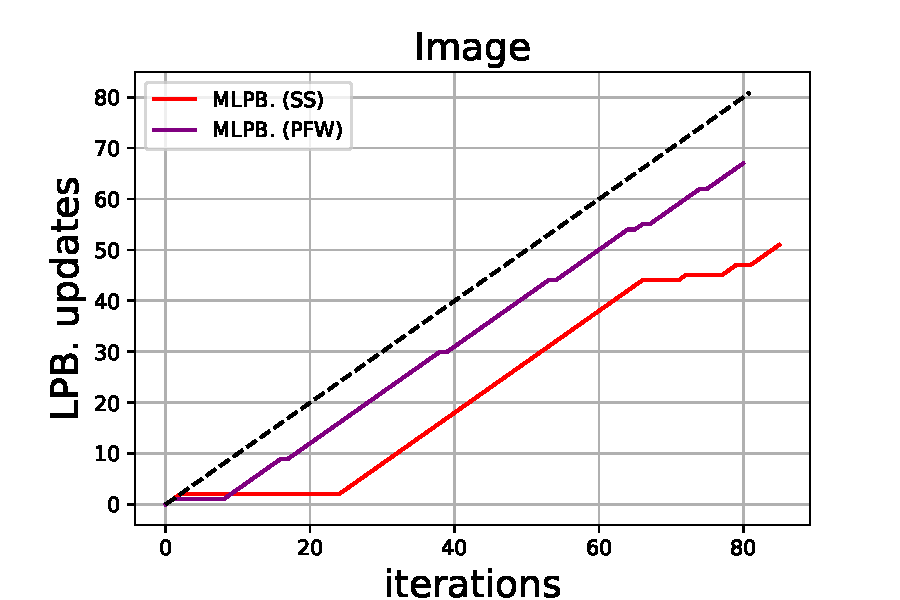
\includegraphics[keepaspectratio, scale=0.30]
            {figure/mlpb_lpb_update_image.pdf}
        \end{minipage}
        &
        \begin{minipage}[t]{0.31\hsize}
            \centering
            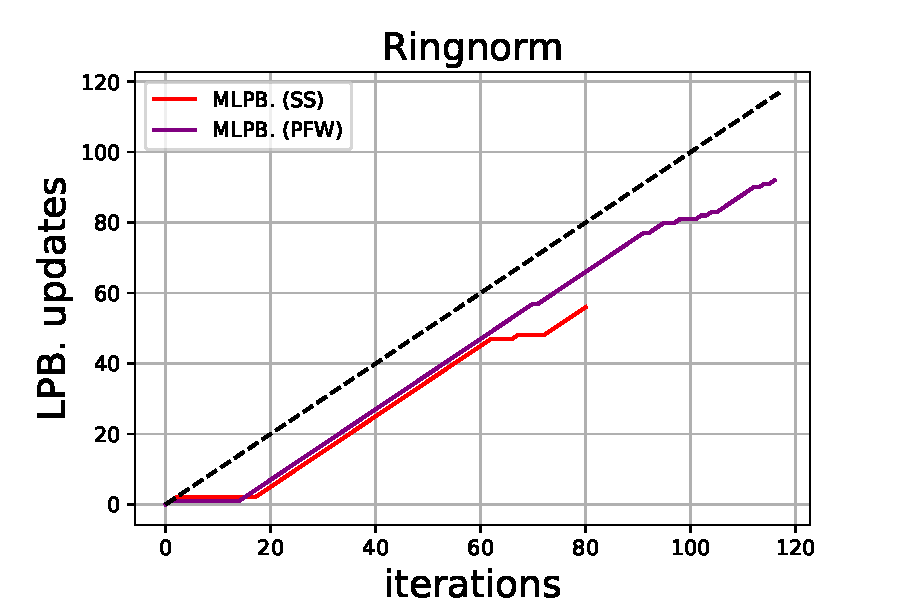
\includegraphics[keepaspectratio, scale=0.30]
            {figure/mlpb_lpb_update_ringnorm.pdf}
        \end{minipage}
        &
        \begin{minipage}[t]{0.31\hsize}
            \centering
            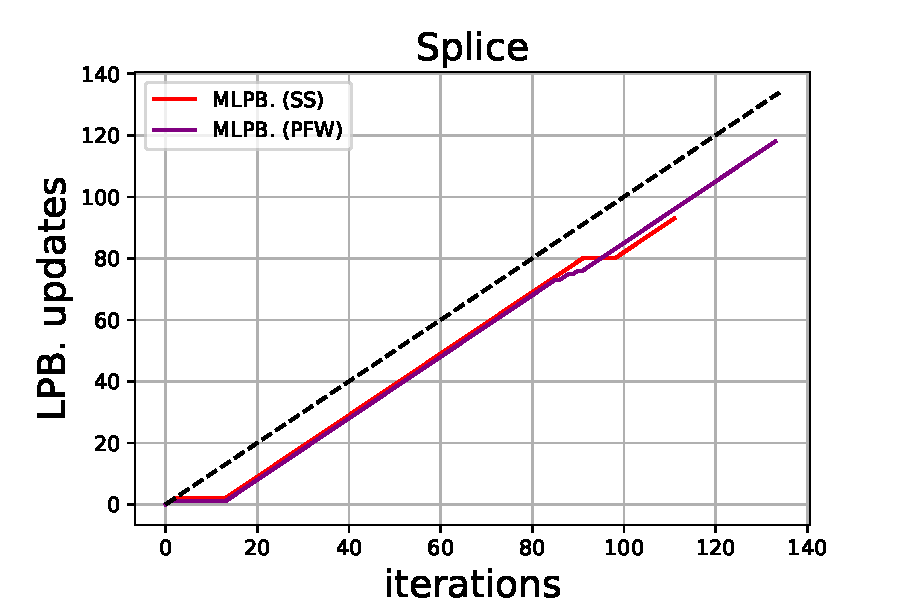
\includegraphics[keepaspectratio, scale=0.30]
            {figure/mlpb_lpb_update_splice.pdf}
        \end{minipage}
        \\
        \begin{minipage}[t]{0.31\hsize}
            \centering
            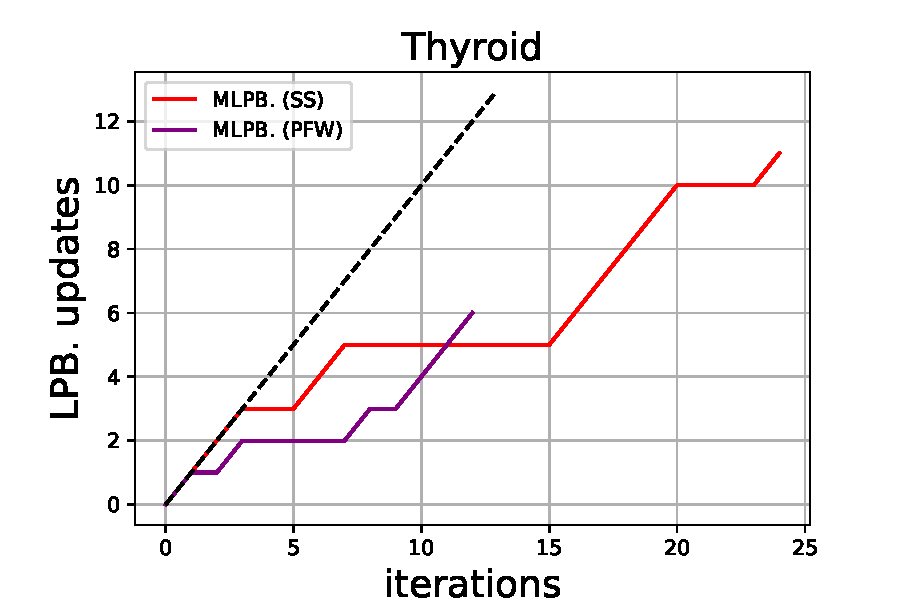
\includegraphics[keepaspectratio, scale=0.30]
            {figure/mlpb_lpb_update_thyroid.pdf}
        \end{minipage}
        &
        \begin{minipage}[t]{0.31\hsize}
            \centering
            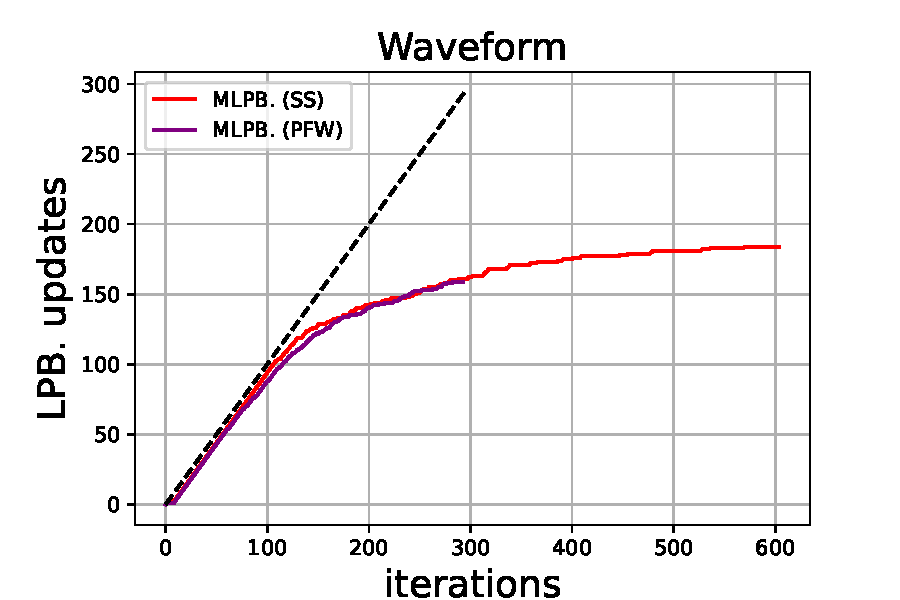
\includegraphics[keepaspectratio, scale=0.30]
            {figure/mlpb_lpb_update_waveform.pdf}
        \end{minipage}
        &
        \begin{minipage}[t]{0.31\hsize}
            \centering
            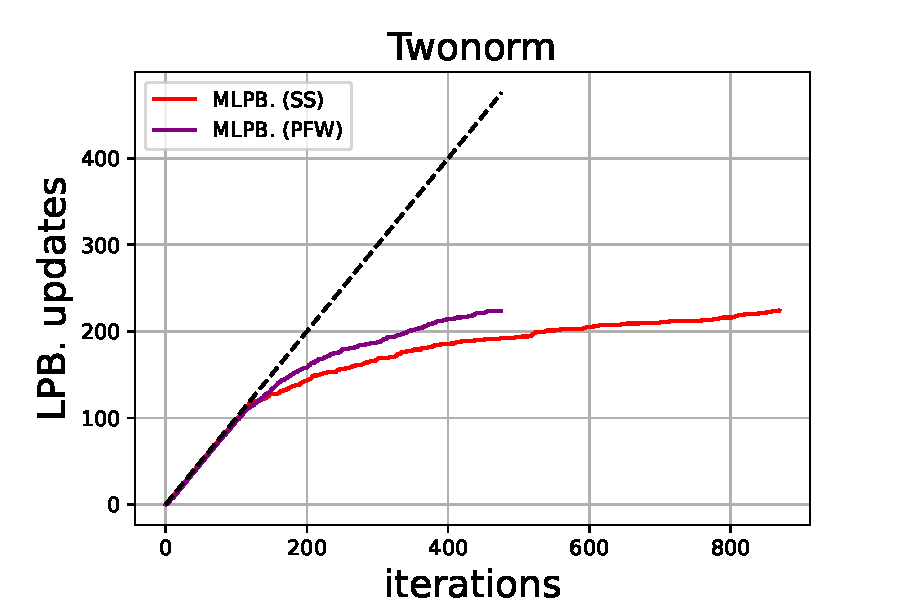
\includegraphics[keepaspectratio, scale=0.30]
            {figure/mlpb_lpb_update_twonorm.pdf}
        \end{minipage}
    \end{tabular}
    \caption{%
        The number of $\secalg$ updates %
        for each benchmark dataset %
        with parameters $\nu = 0.1m$ and $\epsilon = 0.01$. %
        The dotted line indicates the linear function for comparison. %
        Since the shape of the titanic dataset is %
        the same as the F. Solar dataset, %
        we omit it. %
    }
    \label{fig:appendix_lpbcall}
\end{figure}


Finally, we verify the effectiveness of the secondary update $\secalg$, 
shown in algorithm~\ref{alg:lpb_subroutine}. 
For comparison, we measured the soft margin objective and time 
for FW, PFW, MLPB.~(SS), and MLPB.~(PFW). 
FW is the FW algorithm with short-steps, 
and PFW is the Pairwise FW algorithm. 
MLPB.~(SS) and MLPB.~(PFW) are MLPBoosts 
with algorithms~\ref{alg:ss_rule} and~\ref{alg:pairwise_rule}, 
respectively. 
Figure~\ref{fig:appendix_mlpb_compare} shows the results. 
As this figure shows, 
the secondary update $\secalg$ 
improves the objective value significantly. 
\begin{figure}[p]
    \centering
    \begin{tabular}{ccc}
        \begin{minipage}[t]{0.31\hsize}
            \centering
            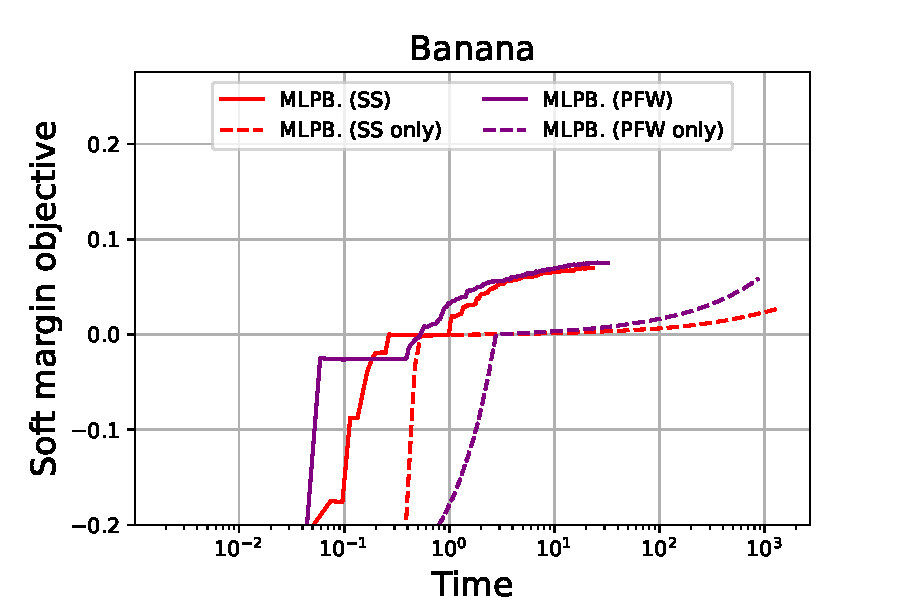
\includegraphics[keepaspectratio, scale=0.30]
            {figure/compare_fw_banana.pdf}
        \end{minipage}
        &
        \begin{minipage}[t]{0.31\hsize}
            \centering
            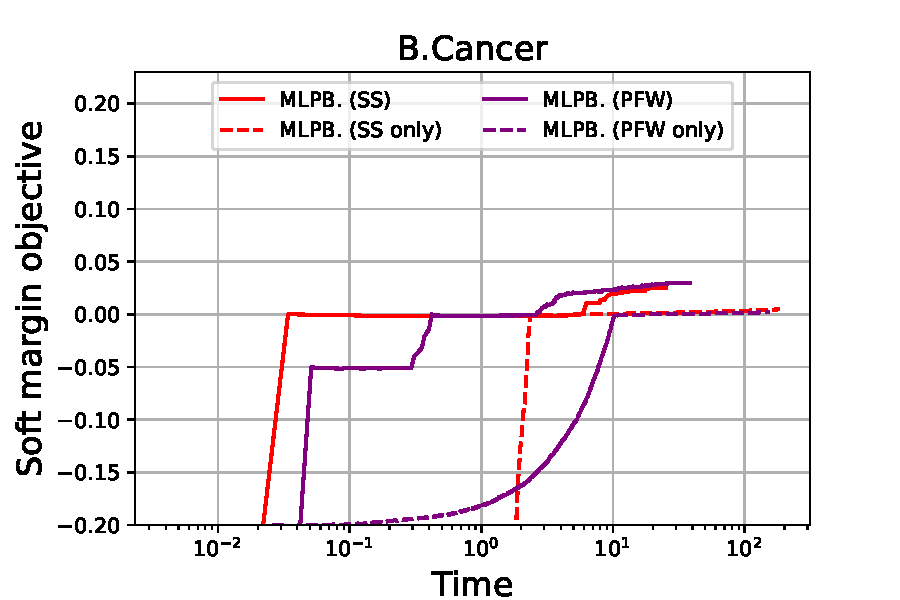
\includegraphics[keepaspectratio, scale=0.30]
            {figure/compare_fw_breast_cancer.pdf}
        \end{minipage}
        &
        \begin{minipage}[t]{0.31\hsize}
            \centering
            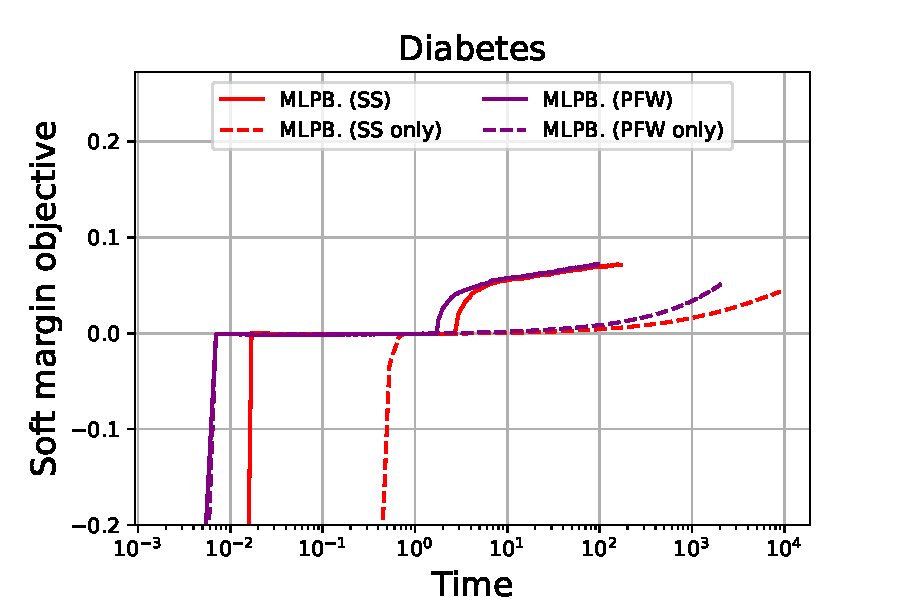
\includegraphics[keepaspectratio, scale=0.30]
            {figure/compare_fw_diabetis.pdf}
        \end{minipage}
        \\
        \begin{minipage}[t]{0.31\hsize}
            \centering
            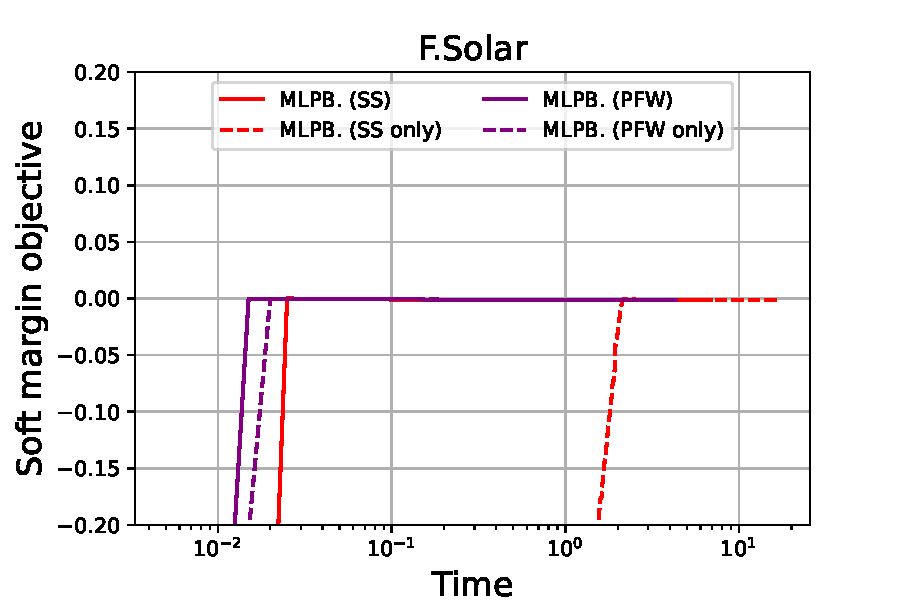
\includegraphics[keepaspectratio, scale=0.30]
            {figure/compare_fw_flare_solar.pdf}
        \end{minipage}
        &
        \begin{minipage}[t]{0.31\hsize}
            \centering
            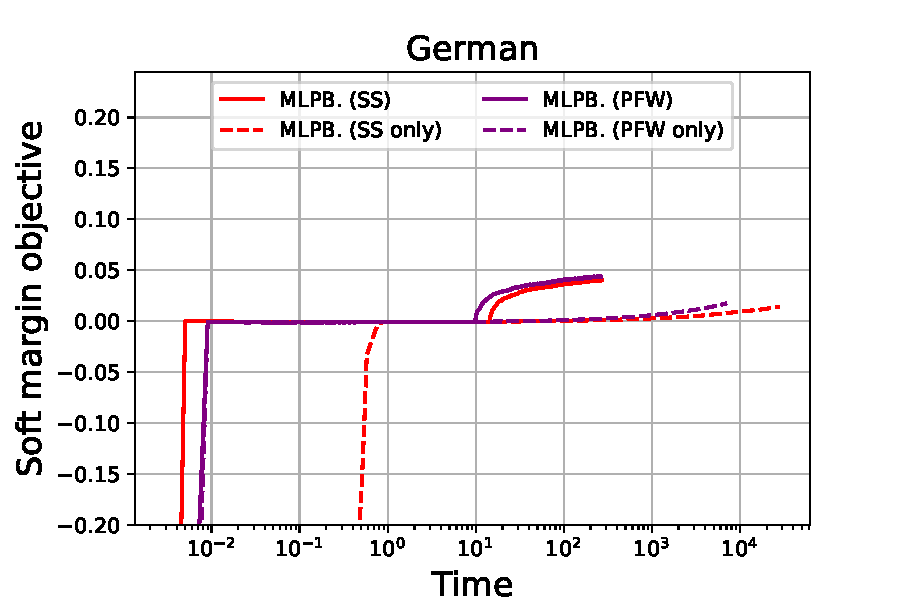
\includegraphics[keepaspectratio, scale=0.30]
            {figure/compare_fw_german.pdf}
        \end{minipage}
        &
        \begin{minipage}[t]{0.31\hsize}
            \centering
            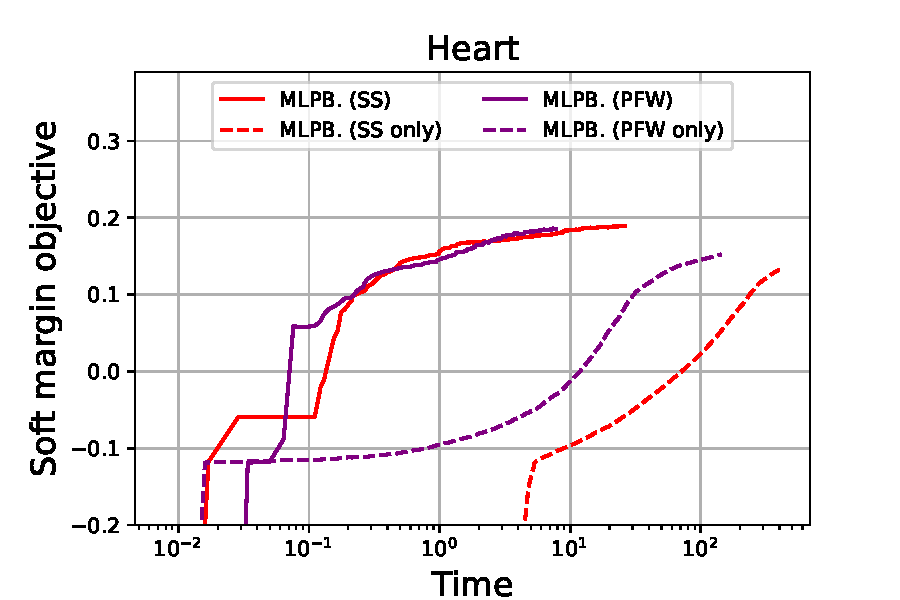
\includegraphics[keepaspectratio, scale=0.30]
            {figure/compare_fw_heart.pdf}
        \end{minipage}
        \\
        \begin{minipage}[t]{0.31\hsize}
            \centering
            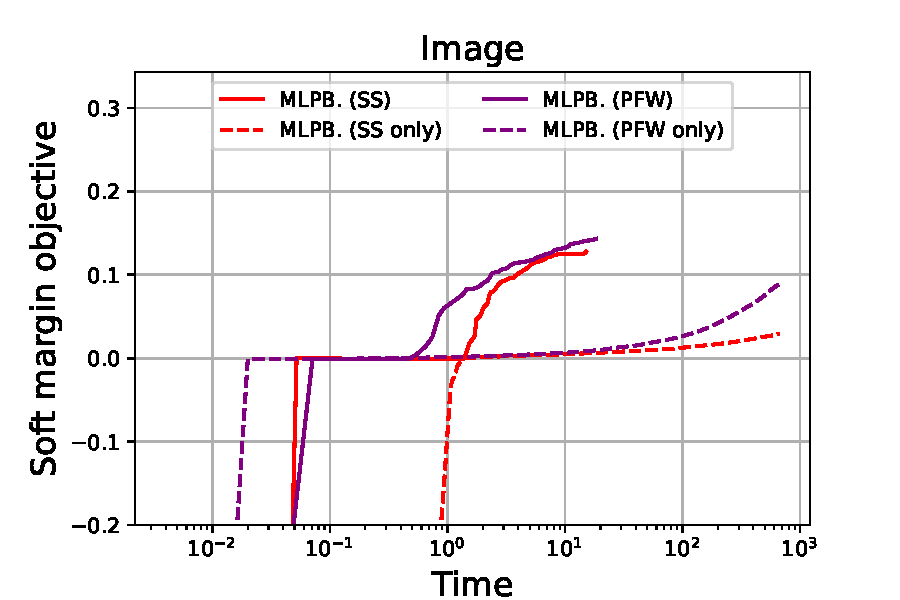
\includegraphics[keepaspectratio, scale=0.30]
            {figure/compare_fw_image.pdf}
        \end{minipage}
        &
        \begin{minipage}[t]{0.31\hsize}
            \centering
            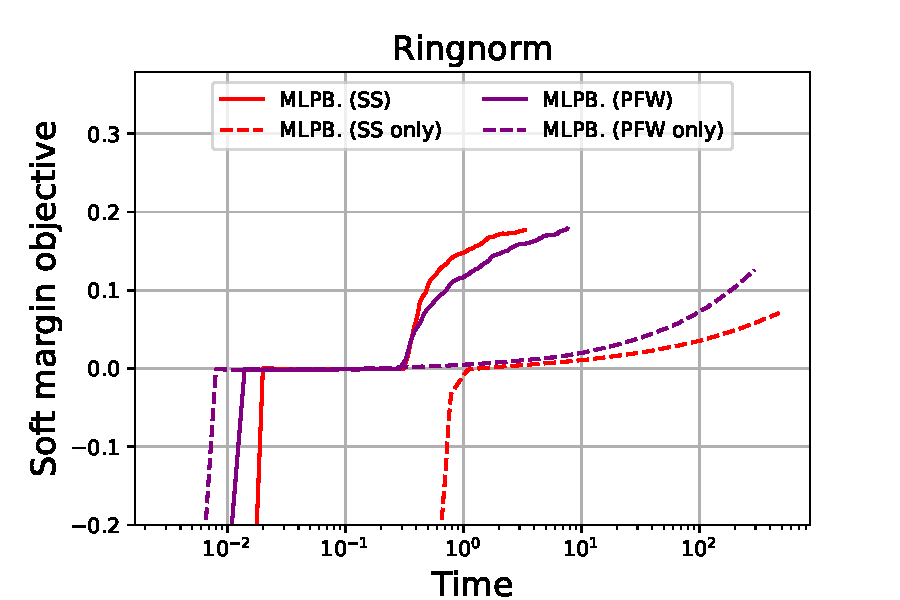
\includegraphics[keepaspectratio, scale=0.30]
            {figure/compare_fw_ringnorm.pdf}
        \end{minipage}
        &
        \begin{minipage}[t]{0.31\hsize}
            \centering
            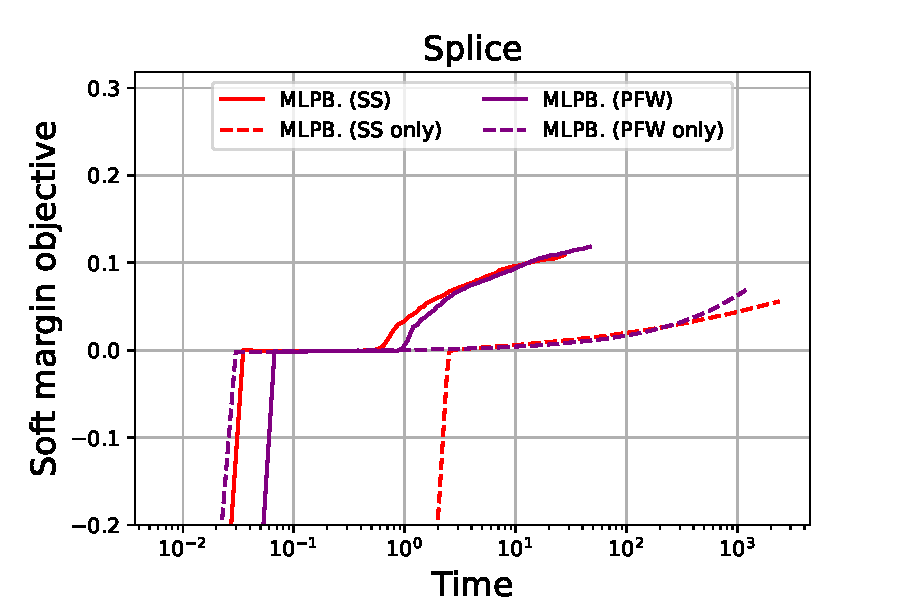
\includegraphics[keepaspectratio, scale=0.30]
            {figure/compare_fw_splice.pdf}
        \end{minipage}
        \\
        \begin{minipage}[t]{0.31\hsize}
            \centering
            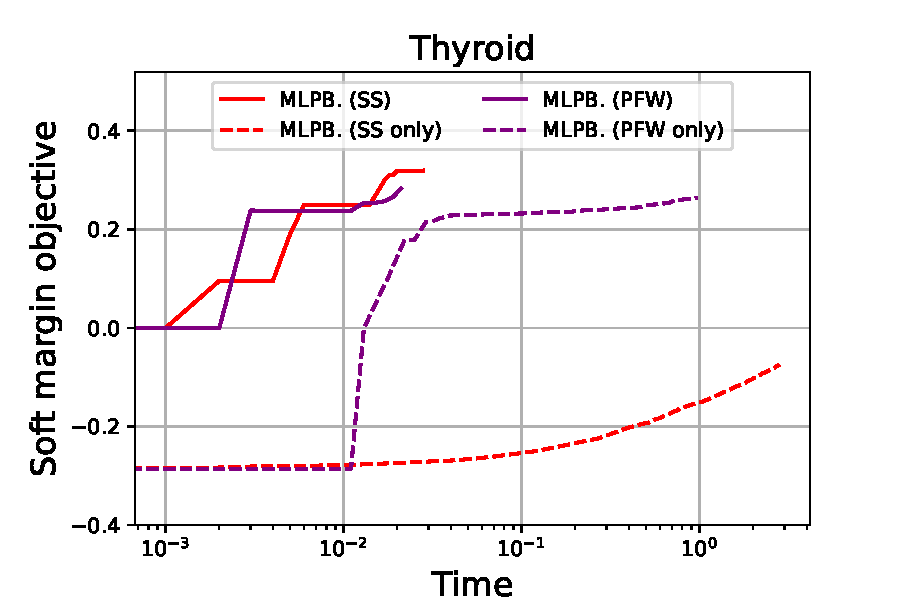
\includegraphics[keepaspectratio, scale=0.30]
            {figure/compare_fw_thyroid.pdf}
        \end{minipage}
        &
        \begin{minipage}[t]{0.31\hsize}
            \centering
            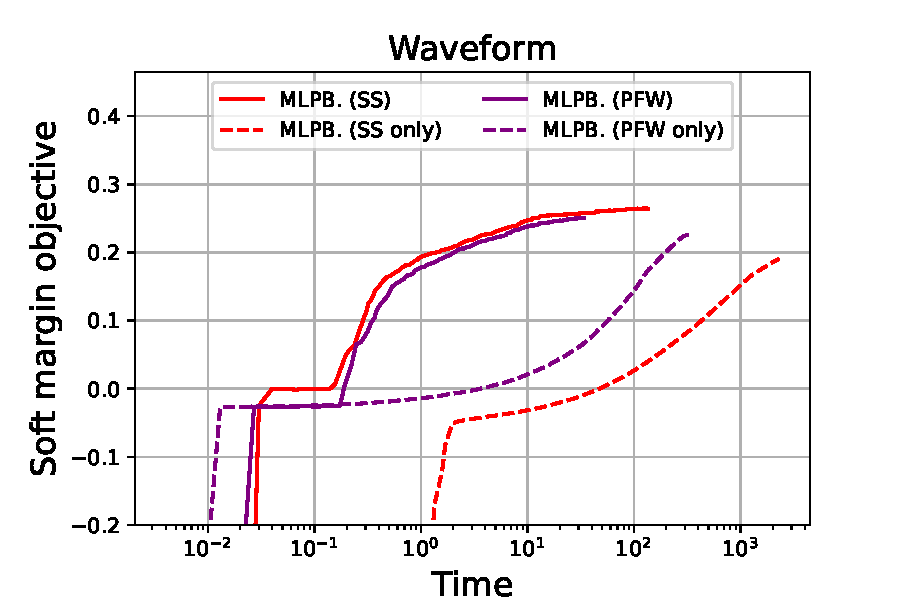
\includegraphics[keepaspectratio, scale=0.30]
            {figure/compare_fw_waveform.pdf}
        \end{minipage}
        &
        \begin{minipage}[t]{0.31\hsize}
            \centering
            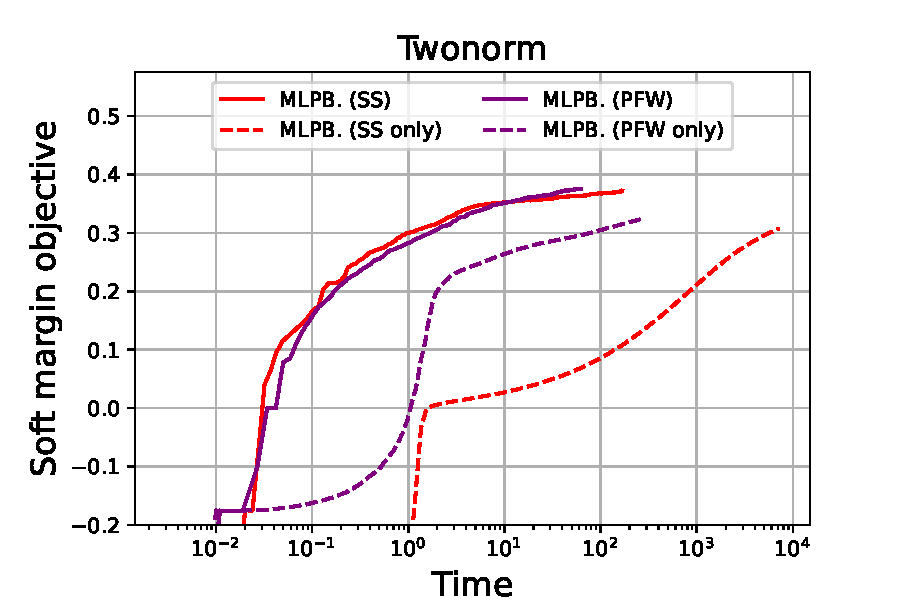
\includegraphics[keepaspectratio, scale=0.30]
            {figure/compare_fw_twonorm.pdf}
        \end{minipage}
    \end{tabular}
    \caption{%
        Comparison of the FW algorithms and MLPBoosts. %
        As this figure shows, the secondary update $\secalg$ yields %
        huge progress. %
    }
    \label{fig:appendix_mlpb_compare}
\end{figure}
